\documentclass[11pt]{article}
\usepackage{amssymb, amsmath,fullpage}
\usepackage{graphicx, setspace,amsthm}
\usepackage{amsfonts,amsmath,amsthm,array,amssymb, mathrsfs}
\usepackage{framed} %%%!!!!!!!!!!!

\begin{document}





\begin{figure}[p]
\centering
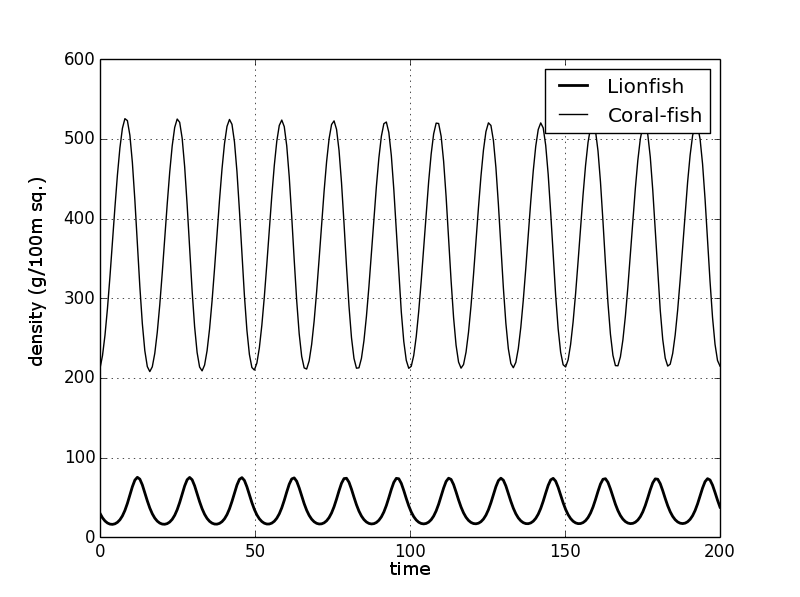
\includegraphics[width=0.8\textwidth]{figure10.png}
\caption{
C0= 212
L0= 5
K= 800
RC=  .447
dl = 0.3
bl= 0.1
hCL=    8.6/240
hLG=  .35
Instability}
\end{figure}


\begin{figure}[p]
\centering
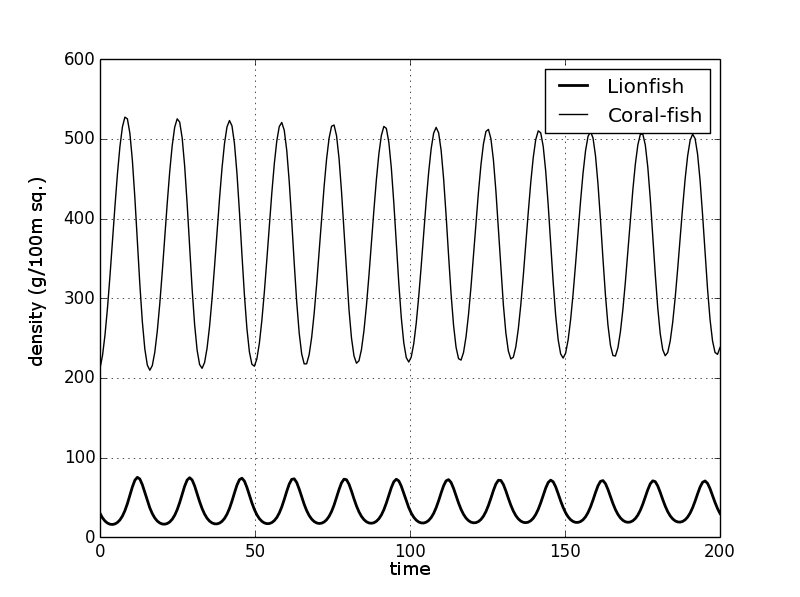
\includegraphics[width=0.8\textwidth]{figure11.png}
\caption{
C0= 212
L0= 5
K= 800
RC=  .447
dl = 0.3
bl= 0.1
hCL=    8.6/240
hLG=  .3525
.35 seems to be the threshold for stability. Next will show 3.49 to show instability}
\end{figure}




\begin{figure}[p]
\centering
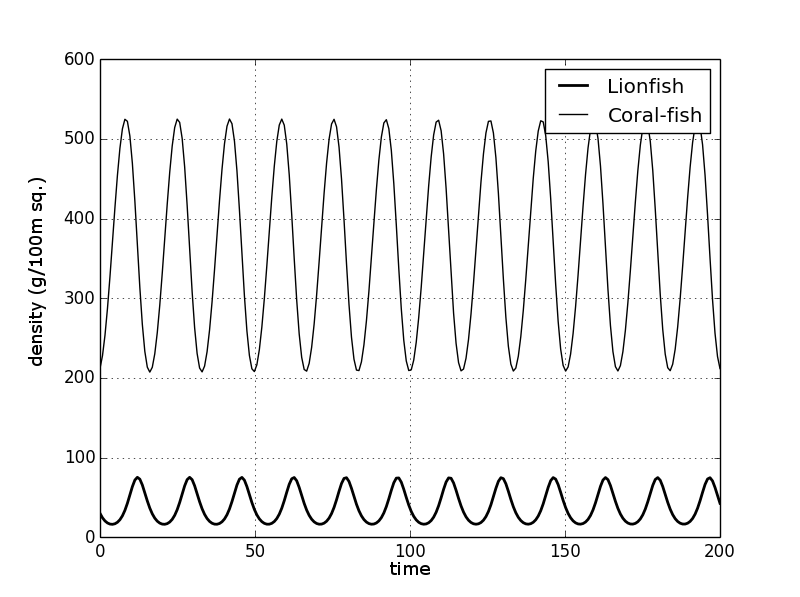
\includegraphics[width=0.8\textwidth]{figure12.png}
\caption{
C0= 212
L0= 5
K= 800
RC=  .447
dl = 0.3
bl= 0.1
hCL=    8.6/240
hLG=  .349
Yep. .35 is the threshold as .349 looks unstable, further with a longer time frame..}
\end{figure}

The three models here are identical except for one parameter. The harvesting rate of lionfish by grouper, ($h_{L,G}$ in the differential model)  is treated as a constant parameter in order to ascertain the approximate harvesting rate needed for the coral-fish population growth to behaved as it did before the arrival of lionfish ({\it locally asymptotically stable}). We observed that coral-fish population behavior change form periodic to $l.a.s$ with larger values of $h_{L,G}$.  This meant that at some value of $h_{L,G}$ the behavior changed, and we varied $h_{L,G}$ in order to find that threshold.  We observed that the change from periodic to $l.a.s$ occurred at very near $.35$ [Figure 1]. To test the validity of our threshold rate we decreased $h_{L,G}$ by .01 (to .349) [Figure 3] and noticed the long term behavior unchanged from Figure 1. Further, we increased our assumed threshold by .0025 (to .3525)[Figure 2] and observed a decreasing amplitude of the solution. Plots done over thousands of months showed that Figure 2 converged and Figure 1 did not. Thus, our harvesting threshold was valid. 

\end{document}